
% Declare document class:
\documentclass[final,3p,times,twocolumn]{elsarticle} % final style
%\documentclass[preprint,12pt,review]{elsarticle} % preprint style


% Declare packages:
\usepackage{amssymb}
\usepackage{graphicx}
\usepackage{setspace} % To control spacing
\usepackage{tabluar}
% Declare journal we're submitting to:
\journal{Journal of Nuclear Materials}


\begin{document}

% Front matter:

\begin{frontmatter}

\title{A superconducting dual-beam cyclotron accelerator based materials test facility for bulk radiation damage studies}

%\author{H.S.~Barnard\corref{cor1}}
%\ead{hbar@mit.edu}

\author{H.S.~Barnard}
%\author{T.~Antaya}
\author{S.E.~Ferry}
\author{J.~Payne}
\author{M.P.~Short}
\author{T.~Sordelet}
\author{R.~Ballinger}
\author{D.G.~Whyte}
% \ead{spad12@mit.edu}

\address{Massachusetts Institute of
  Technology, Dept. of Nuclear Science and Engineering. 
  Cambridge, Massachusetts, 02139,  USA}

%\cortext[cor1]{Corresponding author. Tel.:~;
%  fax:~}

\begin{abstract}

A materials test facility (MTF) utilizing superconducting cyclotron accelerators has been designed to simulate simultaneous neutron damage and helium 
accumulation in materials for fission and fusion applications.  Superconducting cyclotrons can produce high-energy ion beams in small spaces, allowing 
for relatively inexpensive testing of thick ($\sim 1\;\mathrm{mm}$) material samples.  A 35 MeV, 1 mA proton beam is used for simulating atomic 
displacement damage caused by neutrons with damage rates of 50--200 displacements per atom (DPA) per year for various materials.  A 100 MeV He-ion 
cyclotron with an energy degrader is used to produce a variable energy helium beam for simultaneous helium implantation.  Employing high energy beams 
with a range greater than the sample's thickness enables the application of uniform bulk radiation damage, in contrast to heavy ion or lower energy 
proton irradiation studies.  The use of thick samples permits code-approved mechanical testing of macroscopic properties.  The cyclotrons can be 
independently controlled to match the He/dpa ratio to specific environments/neutron spectra or to independently study the effects of He implantation 
and displacement damage.  The novel design for MTF target chamber uses helium-jet impingement cooling to remove heat from multiple samples, allowing 
for steady state operation and in-situ mechanical testing.  Critical issues associated with heat removal, beam material interactions, and operating 
limits are studied to demonstrate the feasibility of the MTF.

\end{abstract}

\begin{keyword}
%% keywords here, in the form: keyword \sep keyword
%% MSC codes here, in the form: \MSC code \sep code
%% or \MSC[2008] code \sep code (2000 is the default)

radiation damage \sep materials testing \sep
accelerators \sep superconducting cyclotron

\PACS 28.52.-s \sep 28.52.Fa \sep 52.40.Hf \sep 52.55.Fa \sep 52.55.Rk
% 28.52.-s Fusion reactors
% 28.52.Fa Fusion reactors - materials
% 52.40.Hf Plasma-material interactions; boundary layer effects
% 52.55.Fa Tokamaks, spherical tokamaks
% 52.55.Rk Power exhaust; divertors
\end{keyword}

\end{frontmatter}

%% main text begins here
\section{Introduction}

%\subsection{Overview of MTF and its Objectives}

%Nuclear energy is receiving increased attention as concern regarding the environmental effects and decreasing supplies of fossil fuel mounts throughout the world.  Unlike other `green technologies, nuclear energy is capable of producing the large amounts of electricity the modern world demands at consistent rates using well-developed technology.

%	Within the nuclear engineering community, there is a growing focus on novel reactor concepts. However, many of these designs - which include fusion reactors, small modular reactors, and fission reactors that utilize high operating temperatures and novel coolants - place demands on structural materials that cannot be met by many of the common materials currently in use within conventional reactor systems. Before any of these innovative technologies can be realized, it must be shown that the proposed structural materials will retain their integrity throughout the operating lifetime.
	
%	A key step in vetting structural materials for future nuclear energy technology will be extensive testing in facilities that can simulate the damaging effects of the proposed reactor on a target material. However, for many of these technologies, the damage rates are expected to be quite high, and there is no existing facility that can simulate damage-over-lifetime on short, research-and-development timescales.
	
The efficient, accelerated study of materials in radiation environments is critical for improving the reliability of modern fission reactors, the 
development of next generation fission reactors, and the eventual development of fusion reactors.  In fission and fusion, neutrons typically damage 
materials through two mechanisms: the displacement of atoms in the material and the accumulation of helium from (n,$\alpha$) reactions and 
$\alpha$-decay of activated nuclei.  These processes depend strongly on the neutron spectrum and the physical and nuclear properties of the material.  
Since neutrons have relatively long mean free paths, the damage occurs within the bulk of material, causing changes to the material's atomic structure 
and leading to macroscopic changes which affect its mechanical and thermal properties. It is this bulk damage that must be accurately recreated during 
accelerated testing for reactor-relevant studies to take place.

The ability to test fission and fusion relevant materials in environments with high neutron fluxes is limited to research reactors [REF], and high 
energy accelerator based techniques such as spallation [REF] and D-T target fusion [REF].  These methods, however, induce radiation damage at similar 
or lower rates than power reactors themselves.  Since most materials in reactors and fusion applications must have lifetimes of several years or 
greater, the development of accelerated methods of testing materials with increased neutron or neutron-like damage rates will greatly benefit the field 
of nuclear material science.

Currently, simulation of neutron damage with ion irradiation is an established technique \cite{Was,ASTME521}.  The ability to dynamically control a 
large (~mA) beam current of protons or helium ions is the key to increasing damage rates compared to neutron irradiation. This allows for accelerated 
radiation damage rates when irradiating materials.  However, these techniques are severely limited by the difficulty of heat removal from samples, and 
are constrained by low energy ($<10\;$ MeV) beams which can only produce near surface ($<250\;\mathrm{\mu m}$) damage in materials.  To simulate 
neutron damage effects, which are nearly spatially uniform through most in-core components, high energy proton beams ($\approx$ 30-40 MeV) are 
required. With recent developments in accelerator technology, it is now possible to achieve these high energies with compact ($\sim$2 m diameter) 
superconducting cyclotrons instead of linear accelerators (10--100m in length).

%***QUESTION: What is the real extractable current from these things? What about the recent 25-30MeV one? Ask Mich State folks about this one.

We propose a novel accelerator based materials test facility (MTF) for simulating concurrent bulk radiation damage and mechanical loading in nuclear 
fuels and structural materials up to $\sim 1\;\mathrm{mm}$ thick.  This facility utilizes advances in superconducting cyclotron technology and two 
independent ion beams provide unparalleled versatility and in radiation damage simulation.  Neutron damage is simulated in samples contained in 
temperature controlled target chamber using helium jet-impingement for sample cooling.  Displacement by inducing displacements with a 36 MeV proton 
beam that penetrates the bulk of the sample.  In addition, a 100 MeV helium beam with an energy degrader allows for a variable energy He source for 
uniform implantation of helium across the sample to induce materials effects associated with helium accumulation within the material.  MTF will 
therefore, allow the testing of nuclear materials in a relatively short amount of time with independent control of the damage mechanisms in a 
temperature controlled, inert gas environment.

%This irradiation facility will allow the testing of advanced materials in a relatively short amount of time. MTF uses superconducting cyclotrons to accelerate two beams, of helium and protons. The helium beam with an energy degrader allows for a variable energy He source for uniform implantation of helium across the sample, to simulate the second materials damage effect that occurs in nuclear reactors.
 
% Protons can be used to simulate neutron damage, provided the Coulombic interaction is taken into account as needed, and they can be accelerated in a compact, superconducting cyclotron to high energies.



%MTF is a versatile design concept that can rapidly simulate effects of neutron damage through proton irradiation. It can also accommodate a wide range of helium implantation rates.  


%\subsubsection*{Design Goals}
%\big

%\begin{enumerate}
%\item Able to allow for the testing of multiple samples 
%
%\item Able to achieve high damage rates in a short amount of time to simulate lifetime damage incurred on a component
%
%\item Capable of simulating damage from helium and neutrons, and possibly heavy ions\footnote{Some sort of third beam, for heavy ion implantation, is being considered as a potential addition.}
%
%\item Sufficiently compact, so that it can be housed in an existing building at MIT, while still maintaining its capability of producing high energy particle beams
%
%\item Able to efficiently cool the samples and provideadequate heat removal at high radiation damage rates.
%
%\item Able to simulate damage in a sample such that the results can be extrapolated to the bulk material.
%
%\item Able to allow for in-situ tensile testing to allow for irradiation under active loads.
%
%\item Capable of irradiating materials such that the temperature distribution across the samples remains within the ASTM standards for accurate materials testing 
%\end{enumerate}
%\bigskip
%
%No dedicated materials irradiation facility currently exists that fulfils each of these objectives. MIT also lacks a facility dedicated to the irradiation of innovative materials. This facility would be of great importance to the capabilities of MIT nuclear materials research, and to the progress of the advanced nuclear materials field in general. 

%\subsection{Overview of this Document} 
%
%This report compiles the results of our investigation into an initial design for MTF. Results that have been improved or corrected since they were initially reported are included in their most current, relevant forms. Our objectives were as follows : 
%
%\bigskip
%\begin{enumerate} 
%\item Create a conceptual design for the MTF facility. This includes the cyclotrons, beam transport, the target chamber, and the sample holders. 
%
%\item Determine an estimation of dpa rates for a variety of likely-to-be-tested materials, in order to show that this facility can provide MIT with the capability of simulating lifetime radiation damage in a material on a short timescale (1 y or less)
%
%\item Design a cooling system and use thermal models to show that it is capable of removing heat from the samples. Show that the sample temperature variation remains within acceptable limits. 
%
%\item Design the "beam window" as a vacuum--helium interface to separate the accelerators/beamlines from the target chamber.
%
%\item Consider the time structure of the beam to ensure that bulk material damage is being adequately simulated. 
%
%\item  Further consider materials that are likely to be tested. What particular properties would need to be accounted for prior to testing? 
%
%\item  Provide a survey of other irradiation facilities to show that MTF provides experimental abilities they cannot.
%
%\bigskip
%
%This work was done as part of the 22.033/22.33 design project class within the MIT Department of Nuclear Science and Engineering. It is our hope that it will provide a useful starting point for further development of the MTF design in the near future. 

\section{Background}

There is a need for a materials testing facility that can accurately, and quickly access material properties. This would be a facility that could achieve at least 40-50+ dpa per year. Currently, there are no fast spectrum and fusion material test facilities. There are two thermal spectrum test facilities (ATR \cite{?} and HFIR \cite{lucas1990review}). The The International Fusion Materials Irradiation Facility (IFMIF) has been proposed for construction within the the next decade. IFMIF uses a high energy deuteron beam and a tritiated (tritium-containing) target to produce fusion neutrons designed to test hundreds to thousands of samples at once. However, the projected costs of IFMIF approach 1 billion dollars and are limited to damage rates on the order of 10-20 dpa per year of operation \cite{?}.

Another option is fission test reactors.  Test reactors have been an valuble reasource for testing in neutron environments, however, due to the time scales involved, high DPA experiments are impractical.  For example, a typical neutron irradiation experiment in a test reactor often requires as much as a year of sample preparation, cooling analysis and capsule design before testing, followed by several years of neutron exposure in the reactor \cite{sickafus2007radiation}. Additional time is needed because of the safety and legal issues of the handling of radioactive materials in the vicinity of a nuclear reactor and because of the high activation level of the irradiated sample and its container. This time period, sometimes up to 5 years, as well as the high overall cost of the test run does not allow for iterations or rapid turn around on experiments. % timely turn around, or the schedule impact of budget variations.  

Accelerator based techniques ion irradiation techniques are also in use because of their many practical advantages over neutron irradiation.  Proton irradiation (or other light ions, decreases induced activation of the test equipment and instrumentation, increases the reliability of the experiment allowing it to be interrupted without disturbing the sample, and in many cases the energy of the ion beam can be variable to adjust the recoil spectrum of the atoms. Most importantly, proton irradiation time, logisticss, and operational costs are substantially less compared to neutron irradiation \cite{Was}.

Ion irradiation can achieve extremely high localized damage rates (often as high as ($>10$ DPA/day), especially with low energy ($<$ 10 MeV) beams.  However, heat removal from samples can be challenging at these high damage rates.  Th low energy ion beams have a limited range, typically $<100\mu$m, over which the damage profile is highly non-uniform and peaks close to the ions' maximum penetration depth.  Though these surface damage studies produce a wealth of useful results, they cannot capture the bulk damage effects that occur on the length scale of a material's grain structure which often dominate the behavior of structural materials. [NEEDS MORE BACKGROUND FROM A MAT-SCI PERSPECTIVE].

Extending the ion-irradiation capabilities to macroscopic scale of $\sim$1 mm, critical importance because it would not only enable testing of samples with damage over multiple grain widths but would also allow for samples that are large enough for test mechanical.  Developing these capabilities while simultaneously incorporating independent helium accumulation and temperature and the ability of in-situ mechanical testing is therefore, the goal the MTF design study.  

\section{MTF conceptual design}
MTF uses two compact superconducting cyclotron accelerators to simulate neutron damage.  A model of the facility concept is shown in Figure \ref{fig:FacilityOverview}.  A 36 MeV proton cyclotron is used for simulating displacement damage.  This beam energy was chosen to allow for nearly uniform displacement damage in the bulk of samples up to 1 mm thick.

To simulate the accumulation of helium, which occurs in reactors as a result of $\alpha$--decay and (n,$\alpha$) reactions, a 100 MeV helium cyclotron is used for implantation.  The helium implantation depth is controlled by reducing the beam energy with an 'energy degrader' such as metallic, actively cooled wedge-plate that is inserted into the beam.

A versatile target chamber holds the samples and allows for independent mechanical testing of multiple samples during irradiation over a wide temperature range.  Two beam lines with quadrupole focusing and magnetic steering are used for the the beam transport system, which is used to converge the beams on the the target samples.  Helium jet impingement cooling is used on both sides of the samples to remove heat from the irradiated region. After the proton beam passes through the samples it slows down and stops within the volume of a helium filled chamber, which minimizes activation and facilitates cooling.

\begin{figure*}[htbp]
\begin{center}
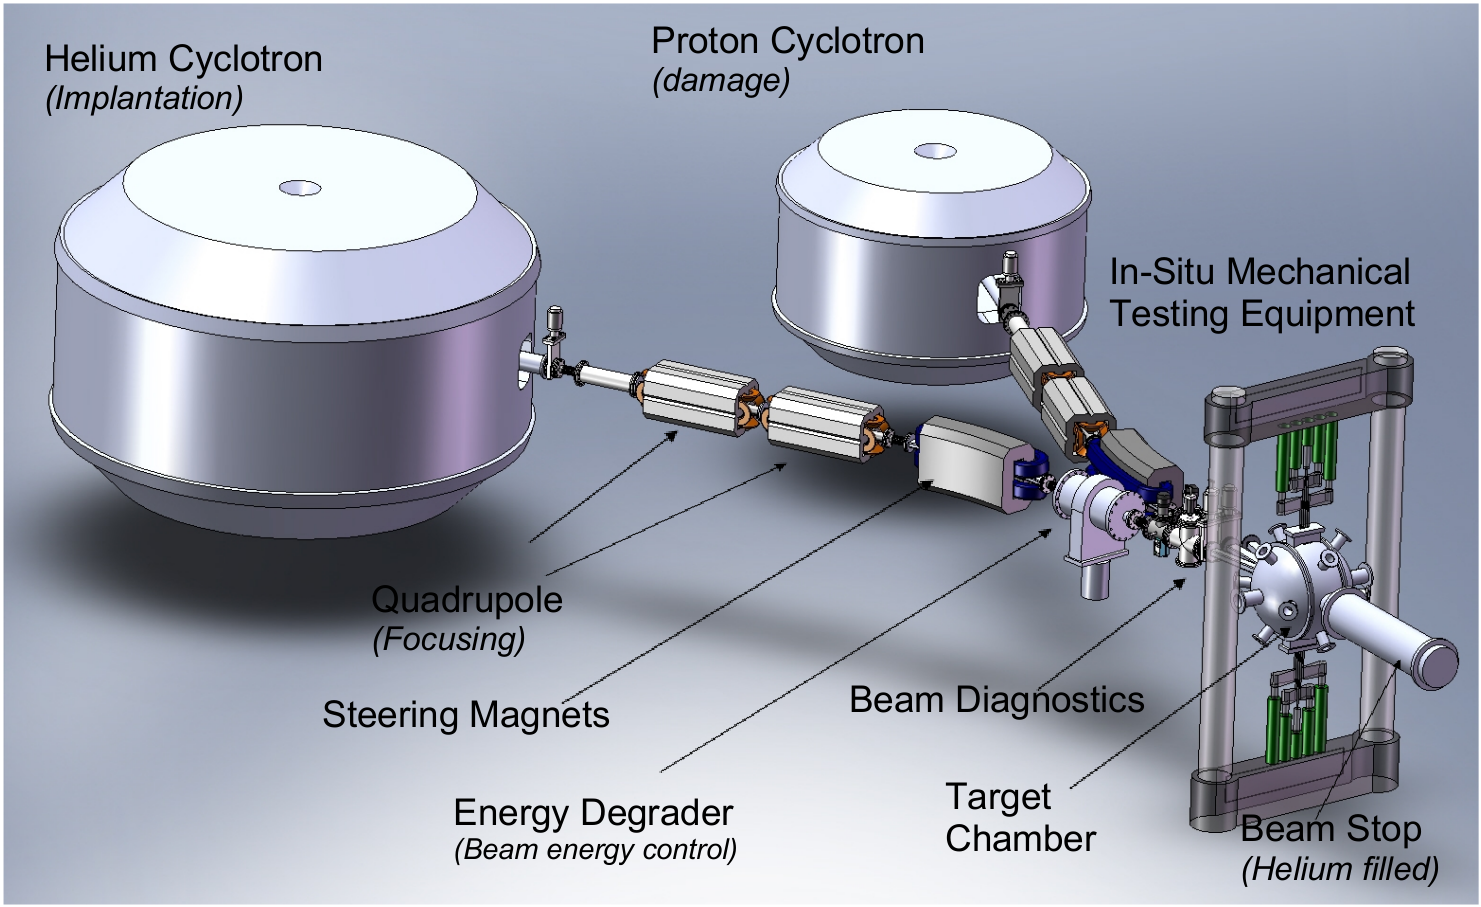
\includegraphics[width=120mm]{Figures/FacilityModel.png}
\caption{The two cyclotrons, for helium implantation and 36 MeV protons, are shown on the left. The beams pass through beam optics and diagnostics. The target chamber is shown on the right, with a beam dump on the far side.  Thermal insulation and coolant piping not shown.}
\label{fig:FacilityOverview}
\end{center}
\end{figure*}

\subsection{Target Chamber}
In the target chamber, samples are mounted in a row and are connected to a test stand that can apply mechanical loads to measure stress-strain properties in-situ or apply loads during irradiation to study radiation-induced creep.  High pressure helium jets are used for cooling the samples that can have volumetric heating from the beam approaching $\sim$20 GW/m$^3$ (20 W/mm$^3$).  Helium is used because it is an established cooling method and because of its favorable qualities as an inert gas that is relatively transparent to ion beams. Helium has excellent thermal properties, high sound speed, and does not become activated by the beam.  Helium is also a noble gas and does not chemically react with the surfaces of the samples, even at high temperatures.  In addition, the beam dump is filled with helium and is integrated into the cooling system to allow beam to slow down and stop after passing through the sample, causing minimal activation outside of the sample.

To separate the pressurized target chamber from the beamlines and the accelerator -- which require a high vacuum environment -- a titanium ($\sim$50$\mu$m) beam window is used as a vacuum/helium interface.  Titanium is used because of it is a favorable balance of high strength and low beam stopping.  A conceptual model of the target chamber is shown in figure \ref{fig:Chamber1} and a cut away schematic of beam and cooling geometry is shown in figure \ref{fig:Cutaway}.  Modeling and analysis of the each of these components are described in the following sections.

\begin{figure}[htbp]
\begin{center}
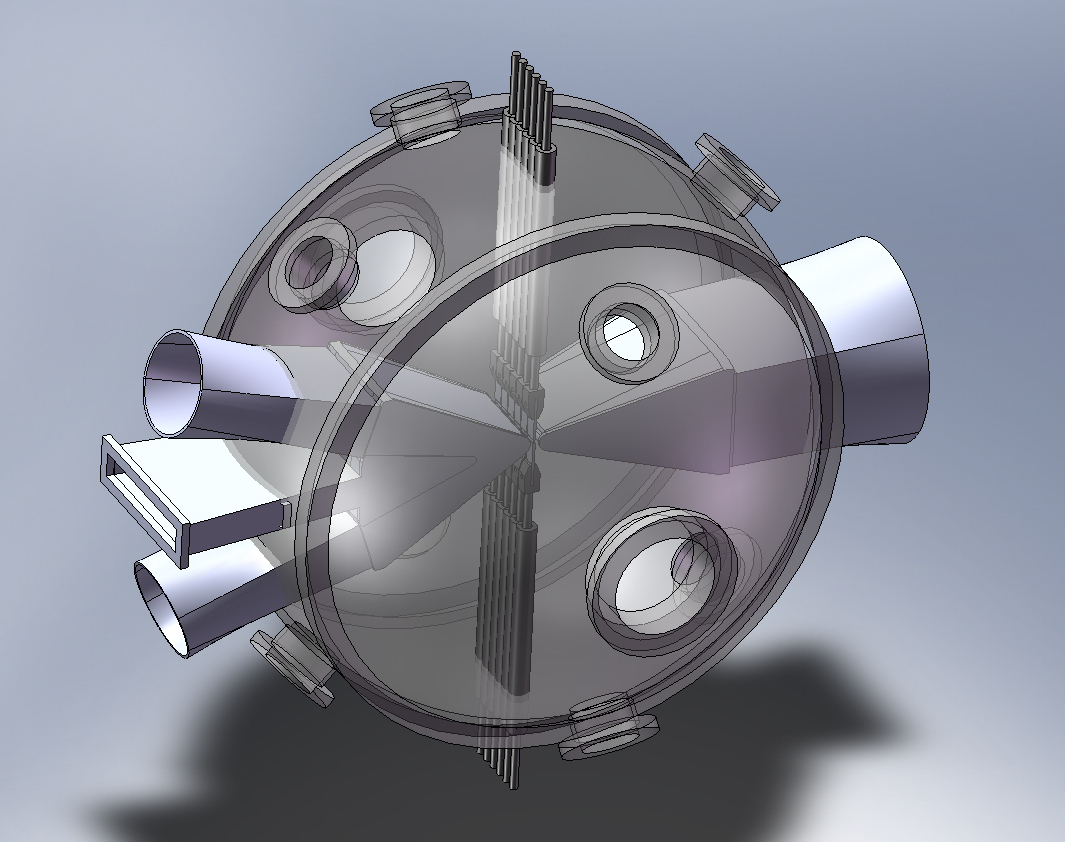
\includegraphics[width=80mm]{Figures/Chamber1.JPG}
\caption{A proposed model of the target chamber is shown. A series of sample holders are held in the center by independent tensile testing actuators.  Manifolds for the helium cooling inlets and beam inlet are shown on the left, and a helium inlet/beam exit is shown on the right.}
\label{fig:Chamber1}
\end{center}
\end{figure}

\begin{figure}[htbp]
\begin{center}
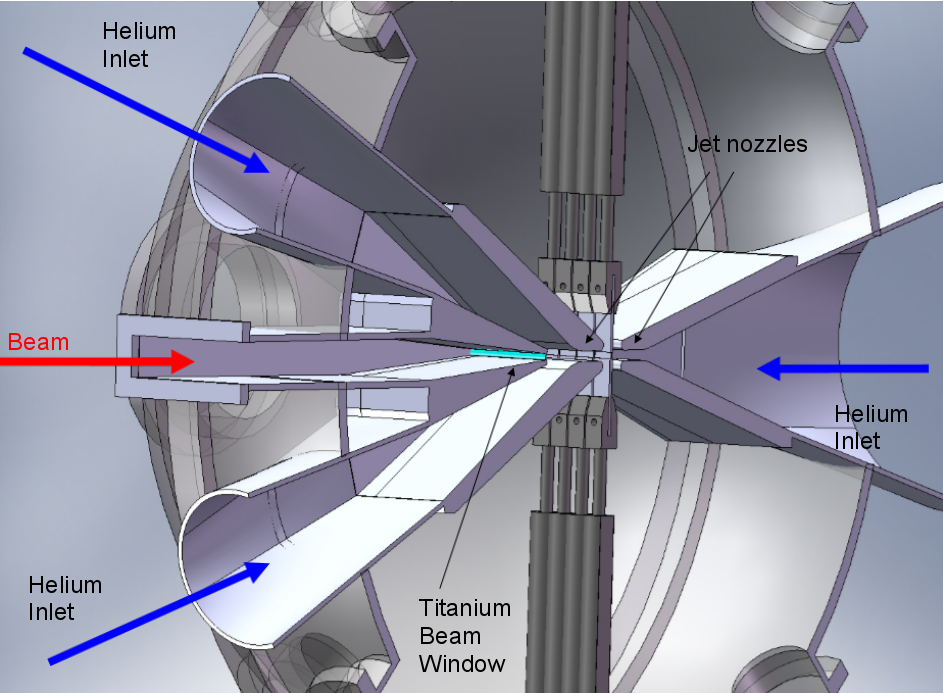
\includegraphics[width=80mm]{Figures/Cutaway.png}
\caption{A cutaway model of the target chamber is shown to illustrate the geometry of the helium gas jets nozzles, samples, and the beam window.}
\label{fig:Cutaway}
\end{center}
\end{figure}

%\section{A proposed initial design for the facility} 

%The facility requires two super--conducting cyclotrons with focusing and steering elements for beam transport.  A 40 MeV proton cyclotron will be used for the to induce damage in samples up to 1 mm with minimal displacement.

%Figure 1 shows a proposed design for the facility, including the cyclotrons, the beam collimators, and the target chamber. Figures 2 and 4 show views of the target chamber; Figure 3 shows a possible design for a sample holder that would allow tensile testing during irradiation. 

%*******************************************************************************

\section{Accelerators and beam parameters}

%	The choice of a 4-5T 36MeV proton and 100 MeV helium cyclotrons was determined by the bounds of the following table. Our goal was to select tested and benchmarked cyclotrons to avoid running into design and operation issues. In the table below there are cyclotron of higher field and energy (Still River PBRT), higher field but lower energy (DTRA Demo), and lower field with high energy (ACCEL-250). The current cyclotrons gave us confidence that an average field, low energy cyclotron could be built successfully. Other issues arise when operating in magnetic fields above 6T. Since the saturation limit of iron is around 2T, maintaining and controlling the stability of the particle becomes difficult for compact machines [Antaya “orbit’]. It was then decided to stay below 6T to avoid implications of design and operational limits.

Isochronous cyclotrons are continuous wave (CW) accelerators allowing for maximum time averaged beam current.  Unlike the classical Lawrence cyclotron, isochronous cyclotron can produce much higher energy beams, into the hundreds of MeV, by increasing the magnetic field radius to account for the relativistic mass increase $B=\gamma B_o$.  There is also flexibility in the design to allow for variable energy and ion species by altering the RF frequency and isochronous field.  Isochronous cyclotrons require an additionally complex magnetic structure for maintain the orbits' phase stability though the design process for these fields is well understood \cite{strijckmans2001isochronous}. Today isochronous cyclotrons are most commonly built cyclotron and are well suited for MTF because of their steady state operation, compact size, and industry experience.

A 36 MeV isochronous proton cyclotron and a 100 MeV isochronous helium cyclotron with 4--5 T B-fields were chosen for the MTF conceptual design.  These design parameters were chosen considering proton beam penetration depth, displacement damage distribution, He implantation depth, and feasibility based on technical experience in cyclotron field. 

\subsection{Proton beam parameters}
Since proton range increases with beam energy while displacement damage rate decreases with energy, the optimal beam energy is achieved at the lowest energy that produces uniform damage in a sample of a given thickness.  Damage rates are also constrained by the desired sample thickness beause cooling requirements that are limited by heat trasfer at the surface and heat conduction within the sample. A proton energy of 36 MeV was chosen to assure adequate penetration of 1 mm samples with a nearly-uniform damage profile while maintaining the a high displacement rate.  This energy was chosen based on calculations of damage profiles and proton ranges, performed using SRIM2008 \cite{SRIM}.  The damage profile caused by 36MeV protons in 304 stainless steel is shown in figure \ref{fig:FeRange}.

\begin{figure}[htbp]
\begin{center}
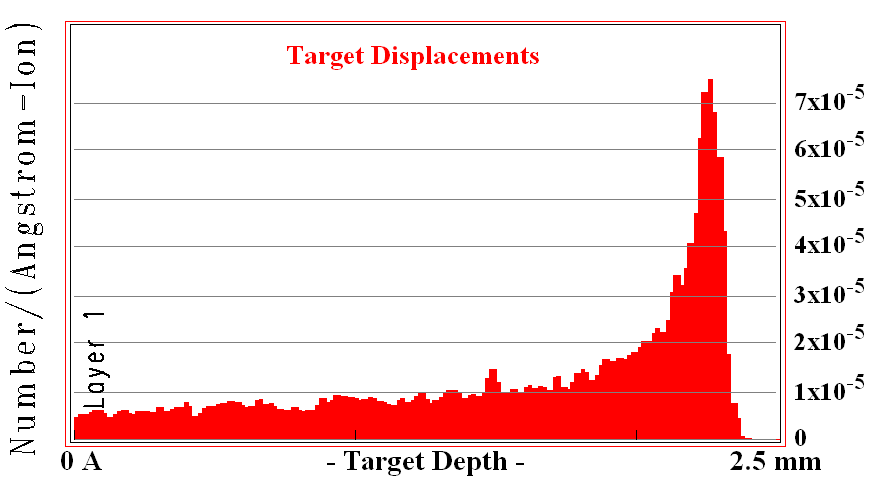
\includegraphics[width=80mm]{Figures/FeRange.png}
\caption{Displacement profile for protons in 304 Stainless Steel generated with SRIM2008.  Nearly uniform bulk damage is observed in the first 1 mm of the proton range.}
\label{fig:FeRange}
\end{center}
\end{figure}

The achievable beam current sets a fundamental limit on the sample volume that can be studied.  As beam current increases, the achievable beam current densities on the sample quickly exceed the heat removal limits.  For example, even with relatively low average beam current ($<$0.1 mA), a 1 mm thick, 1 cm wide sample, heat removal is primary constraint on induced the DPA rate, as shown in section \ref{sec:OperatingConstraints}.  The total current however is very import because, by sweeping the beam across many samples, the average beam current density can be adjusted to maximize the damage rate over a maximum number of samples.  

Compact high current cyclotron pose several technical challenges that limit the maximum beam current.  As the magnetic field is increased to make the cyclotron smaller, the field gradients in the radial direction must increase to maintain the proper fields for isochronous acceleration. This causes the orbits to be in close proximity, requiring the beam to have very small transverse dimensions.  High current and small beam size makes beams stability more problematic and close orbits makes beam extraction more substantially more difficult.  

For this study, a range of 0.1 - 1 mA of beam current is assumed.  Since optimization of the for high beam current and extraction involved a detailed design of the cyclotron, the bounds of this range were estimated from industry experience.  Currents on the order of 0.1 mA have been readily achieved by superconducting cyclotrons on this scale \cite{???}.  The upper bound is more difficult to determine, however, since isotope production cyclotron have achieved reliable beam currents exceeding 2 mA \cite{Jongen201047} \cite{???} at slightly lower fields, $\sim$1mA was chosen as a conservative upper limit than can be achieved without substantial R\&D efforts.




%\subsection{Beam Current}
%\begin{itemize}
%\item Ion sources and available technology ?
%\item Current limitations due to space charge expansion? 
%\item Current limitations due to Challenges with extraction ?
%\end{itemize}
%
%................................................................................\\
%................................................................................\\
%................................................................................\\
%................................................................................\\
%

\section{Helium Implantation}

The accumulation of helium in irradiated materials from $\alpha$ decay and (n,$\alpha$) reactions contributes significantly to embrittlement and swelling of materials.  Helium implantation is therefore a very important feature of MTF.  Helium implantation is achieved in samples up to 1 mm thick with a 100 MeV cyclotron because helium ions with this energy have ranges of greater than 1 mm for most materials.  An energy degrader is used to reduce the beam energy to vary the implantation depth, which allows for a uniform helium profile.

The helium/DPA ratio has a strong dependence on the materials nuclear properties and the neutron spectrum.  Since a separate cyclotron is used for helium implantation, the helium/dpa ratio is highly flexible and can be adjusted to match the helium/dpa ratios for practically any known fission or fusion materials application.  The annual He accumulation is shown for several reactor applications in table \ref{tab:AnnualHe}.

\begin{table}
\begin{center}
\caption{Annual Helium accumulation}
 \begin{tabular}{|c|c|}
  \hline
 & He Accumulation \\ 
    Material type & [appm/year] \\ \hline
   Metals (fusion)   	& $\sim$200               	\\
   Graphite/SiC (fusion) & $>$1000                 	\\
   Metals (fission)  	& 10-100                  	\\
  \hline
 \end{tabular}
\caption{Estimates of helium accumulation rates for materials in reactor relevant environments \cite{huh}} 
\label{tab:AnnualHe}
\end{center}
\end{table}

\subsection{Implantation Rate}
The helium implantation rate can be calculated directly from the helium beam current density with equation \ref{eq:HeRate1}.  The He implantation rate can also be calculated in atomic parts per million per hour [appm/hour] as shown in equation \ref{eq:HeRate2}.

\begin{equation}
\Phi_{He} = \frac{J_{He}}{q_o} \quad \longrightarrow \quad R_{\mathrm{He}} [\mathrm{He/s}] = \frac{\Phi_{He}}{\Delta x}
\label{eq:HeRate1}
\end{equation}

\begin{equation}
R_{He} [\mathrm{appm/hr}] = \frac{(3.6\times 10^9)\cdot J_{He}[\mathrm{A/m}^2]} {e[\mathrm{coul}]\cdot n_t[\mathrm{m}^{-3}]\cdot \Delta x [\mathrm{m}]}
\label{eq:HeRate2}
\end{equation}

\subsection{Accelerated He implantation}
At high temperatures, defects caused by radiation damage can be annealed.  Thermal annealing is seen by many materials, including steels \cite{KluehTwo}, silicon carbide \cite{SneadZinkleTwo}, and tungsten \cite{Lassner}.  This means that for materials at high temperature, it is possible to simulate radiation damage at much higher rates with only helium implantation, assuming the removal displacement damage effects by annealing.  For intermediate temperatures, it might also be sufficient to amorphize the material with several proton induced DPA followed by rapid He implantation.  This mode of operation could be extremely advantageous because it would enable end-of-life material studies to be performed orders of magnitude faster than proton induced DPA studies. 

Since all of the energy of implanted ions is the deposited in the material, the main challenge at high implantation rates is volumetric heating.  The volumetric heating can be calculated from the time averaged beam energy $\bar{E}$ from equation \ref{eq:EBar}, where $E(t)$ must be calculated to create a uniform deposition profiles from inverse range data $[R(E)]^{-1} = E(R)$, where R(E) can be calculated from SRIM 2008 \cite{SRIM}.  An expression for a sinusoidally varying range sweep for implantation, $E(t)$ is given by equation \ref{eq:ESweep}, where $\omega$ is the range sweep frequency.

\begin{equation}
\bar{E} = \frac{1}{\tau}\int_0^\tau E(t)dt \quad
\label{eq:EBar}
\end{equation}

\begin{equation}
E(t) = E(R(t)) , \quad R(t) = \frac{\Delta x}{2} (1 +\sin(\omega t))
\label{eq:ESweep}
\end{equation}

The average volumetric heating $q'''$ is therefore is estimated by $q''' = J \cdot \bar{E} / \Delta x$, where $J$ is the current density and $\Delta x$ is the thickness.  To simplify the calculation, $\bar{E}$ can be approximated as the energy required to implant at the maximum depth, divided by 2.  Using this simplification, the maximum hourly rate for helium implantation in atomic parts per million normalized to surface heat flux is shown in Figure \ref{fig:HourlyHeImplantation}.  Since 1 MW/m$^2$ is only a modest heat removal rate for He jet impingement cooling, annual He accumulations (table \ref{tab:AnnualHe}), or even end-of-life accumulation, can be simulated in a matter of hours or days.

%\begin{figure}[htbp]
%\begin{center}
%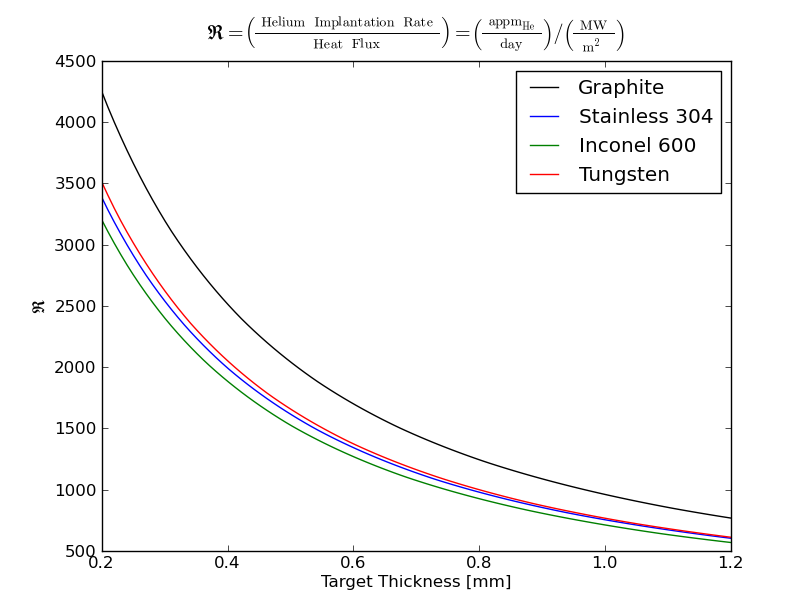
\includegraphics[width=80mm]{Figures/HePerDay.png}
%\caption{Daily helium implantation rate normalized to surface heat exhaust}
%\label{fig:DailyHeImplantation}
%\end{center}
%\end{figure}

\begin{figure}[htbp]
\begin{center}
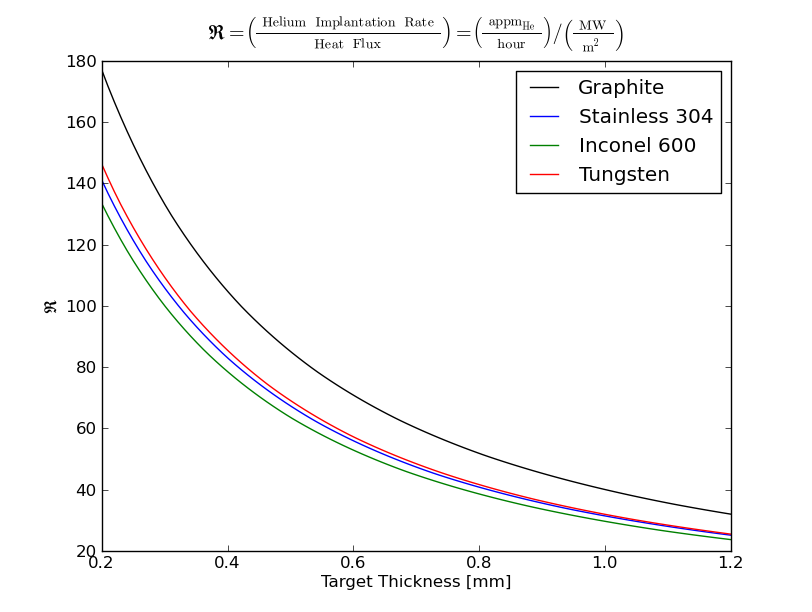
\includegraphics[width=80mm]{Figures/HePerHour.png}
\caption{Hourly helium implantation rate normalized to surface heat exhaust}
\label{fig:HourlyHeImplantation}
\end{center}
\end{figure}


\section{Cyclotron Design}

Beams with high time--averaged current are desirable for damage simulation.  Isochronous cyclotron designs are used because they are continuous wave (CW) devices are have been demonstrated in energy ranges spanning to those required by MTF.  Table \ref{tab:cyclotrons} show a comparison of other isochronous cyclotrons that have been designed built and operated with high reliability for medical and radiation source applications.  MTF is well within the range of available superconducting cyclotron technology and therefore should not require significant R\&D efforts beyond the cyclotron design process and is expected to not pose significant technical risk.  

\begin{table*}
\begin{tabular}{|c|c|c|c|c|} 
\hline Cyclotron & Energy (particle) & B-Field (magnet) & Use & Ref. \\ 
\hline
\hline ACCEL-250 & 250MeV (i) & 2.4T (SC) & PT & \cite{geisler2007commissioning} \\ 
\hline C-230.235 (IBA) & 235MeV (p) & 1.739--2.165T (Cu) & PT & \cite{huh} \\
\hline C-400 & 265MeV(p), 400MeV(i) & $\sim$3.5T (SC)  & PT & \cite{Jongen201047} \\ 
%\hline MYRRHA (IBA) & 40-70MeV,  \cite{abderrahim2001myrrha}
\hline TRADE (IBA) & 110 MeV (p) & (SC) & NS & \cite{jongen2004new}\\
\hline \textbf{Proposed MTF} & \textbf{36MeV(p), 100MeV(He)} & $\sim$\textbf{4T(p), 4T(He) (SC)} & \textbf{MTF} & -- \\ 
\hline DTRA Demo & 10MeV(p), 5MeV(d) & 7T (SC) & DTRA & \cite{huh} \\ 
\hline %Still River PBRT & 250MeV(p) & 9T (SC) & synchronous & PT & \cite{huh} \\ 
%\hline 
\end{tabular} 
\caption{Table of existing isochronous cyclotron designs and facilities.  The design parameters for MTF are within the range of other demonstrated cyclotron facilities.  The MTF's accelerators are therefore feasible without substantial R$\&$D.  The following abbreviations are used: Proton Therapy (PT), Material Test Facility (MTF), Neutron source (ns), Detection Threat Reduction Agency (DTRA), Superconducting(SC), Copper (Cu)}
\label{tab:cyclotrons}
\end{table*}

A study of compact high-field cyclotrons was performed to assess the feasibility of proton and helium cyclotrons for MTF in addition to a preliminary design for beam transport system was developed by T.C. Sordelet, et al \cite{sordelet2011design}.  Several codes were used for this analysis. Poisson Superfish \cite{superfish1976software}, a 2D electro-magnetic field solver, was used to determine general design parameters such cyclotron's size and the basic characteristics of the coils, conductor, resonator, and other components.  

The cyclotron design was further refined with ACFIELDS \cite{block2011}, a semi-analytic cyclotron design code and OPERA 3D \cite{fields2004opera}, a finite element analysis code for electromagnetic field calculation and particle tracking.  Numerous designs for superconducting isochronous cyclotrons were studied, ranging from 3 to 7 Tesla.  These designs involved optimization of the isochronous fields with spiral magnet pole tips for transverse stabilization, coil positioning, and yoke design.  It was concluded that most cost effective compact cyclotrons, posing the least technical risk were designs with average magnetic fields of 4.2T(proton) and 3.9T(helium), niobium titanium (NiTi) superconductors, and iron poles and magnetic return yokes.  The final design parameters concluded from the cyclotron study \cite{sordelet2011design} are given in table \ref{tab:CyclotronParameters}.  These parameters serve to provide an estimate of the physical scope of these accelerators so that costs and facility layout can be assessed in the final design based on available fabrication resources and procurement options.

\begin{table*}
  \begin{tabular}{|l|l|l|l|l|l|l|l|l|} 
    \hline Ion & Type & Energy & Field $\bar{B}$ & $R_{ext}$ & Dimensions & Fe Mass & NiTi Mass \\ 
    \hline
    \hline H$^+$ & isochronous & 36 MeV & 4.2 T & ???? cm & 46cm $\times$ $\O 84$cm & 1372 kg & 18.70 kg   \\
    \hline He$^+$ & isochronous & 100 MeV & 3.9 T & ???? cm & 100cm $\times$ $\O 180$cm & 12728 kg & 81.22 kg  \\
	\hline
  \end{tabular}
\caption{Parameters for MTF cyclotrons to provide an estimate of the physical scope of their designs \cite{sordelet2011design}.}
\label{tab:CyclotronParameters}
\end{table*}


\section{Beam Extraction and Transport}

Positive ions are most commonly extracted by an electrostatic deflector. The electrostatic detector consists of two electrodes located at the extraction radius of the cyclotron \cite{strijckmans2001isochronous}.  This method is possible though efficient extraction becomes difficult when the spacing between ion orbits is small.  Another possiblitiy is negative ion stripping, whereby, negative ions are accelerated then pass though an electron stripping target at maximum orbit radius.  When the electrons are stripped the, now positive, ion is deflected out of the cyclotron.  For high current beams, this method may be problematic due heating and activation of the stripping target or negative ion source limitations. Yet another possibility self-extraction whereby, a magnetic field pertubation is incorporated into the design of the magnet such that ion at the maximum acceleration radius enter unstable orbits and extract themselves.  All of these methods are possible however, a detailed analysis beyond the scope the preliminary design would have been necessary, so further investigation will be required to determine the most efficient method to extract of beams with currents greater than 0.1 mA. [MORE CITATIONS NEEDED].

For transport of the beam from the accelerators to the target chamber, a preliminary design was developed using TRANSPORT \cite{brown1973computer} and is described futher in \cite{sordelet2011design}.  The beam transport system requires only standard components: magnetic quadrupole triplets for focusing and sector magnets for steering and combining the beams.

The details of energy degrader design, used for varying the beam, has been left for future investigation.  The design will likely consist of using a rotating
step or wedged wheel, a movable wedge, or a stack of foils [ASTM E942-96, 2011]. Heat removal will be also be required for the design, however, the thermal requirements will not be any more severe than the inside of the target chamber and are therefore expected to have a straight forward engineering solution. Also, there is considerble experience with energy degraders in the field for medical irradiations and several choices of materials for the degrader are accepted in practice by ASTM E942-96 such as aluminum, beryllium, and graphite which can be incorporated into the design.

\section{Operational Range} 
\label{sec:OperatingConstraints}
As the beam passes through the sample it induces damage, but it also loses energy in the sample, which causes significant volumetric heating.  Volumetric power deposition $q'''$ can be calculated with equation \ref{eq:BeamPower} where $J$ is the beam's current density and S is the beam's stopping power ($S(E) \equiv dE/dx$) for which values are available semi-empirically from SRIM \cite{SRIM}.

\begin{equation}
q''' [W/m^3] = J[A/m^2] \cdot S[eV/m]
\label{eq:BeamPower}
\end{equation}

The heating of the samples results in the two primary constraints on the damage rate: heat removal and the temperature variation across the samples.  It is therefore useful to consider the damage rate that has been normalized to volumetric heating,  shown in figure \ref{fig:DPAvsHeating}.  This plot demonstrates that the achievable damage rates depend strongly on the materials and are relatively insensitive to the beam energy.

\begin{figure}[htbp]
\begin{center}
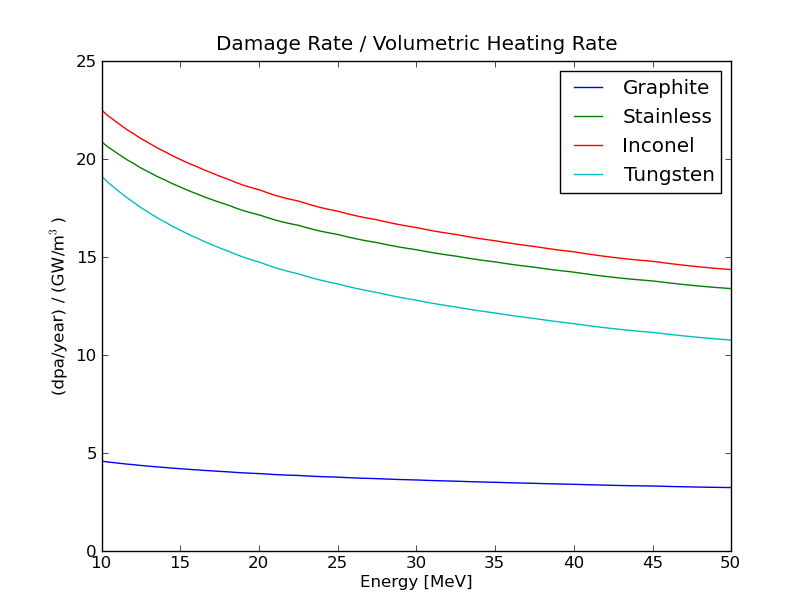
\includegraphics[width=80mm]{Figures/DPAvsHeating.png}
\caption{Damage rates normalized to volumetric heating for various materials.  This shows that the achievable damage rates are relatively insensitive to beam energy and depend strongly on the materials.}
\label{fig:DPAvsHeating}
\end{center}
\end{figure}

For the heat removal constraint, the maximum heat removal rate is set by the surface heat flux $q''$, which is determined by the heat transfer coefficient $h$ as applied in equation \ref{eq:Convection}.  A more detailed calculation and discussion of the heat transfer coefficient is given in Section \ref{sec:HeatRemoval}.  

\begin{equation}
q'' = h \cdot (T_{surface} - T_{coolant})
\label{eq:Convection}
\end{equation} 

From equation \ref{eq:Convection}, for a fixed inlet temperature, the maximum achievable $q''$ increases roughly linearly with sample temperature (with a small correction for the temperature dependence of $h$).  Since the bulk of the sample is heated volumetrically, $q''$ increases linearly with the thickness. The maximum damage rate will therefore decrease roughly linearly with thickness.

A simultaneous operating constrain is the temperature profile within the sample, which is set by the thermal conductivity $k$.  Since material properties can be highly sensitive to temperature, it is necessary minimize the temperature variation $\Delta T$ across the sample.  Equation \ref {eq:MaxT} derived from a simple 1-D slab which can be used to approximate $\Delta T$ for volumetric heating $q'''$ and heat flux $q''$ (on both sides of the sample).

\begin{equation}
\Delta T = \frac{q t^2}{2 k} %=  \frac{q t}{4 k}
\label{eq:MaxT}
\end{equation}

%\begin{figure}[htbp]
%\begin{center}
%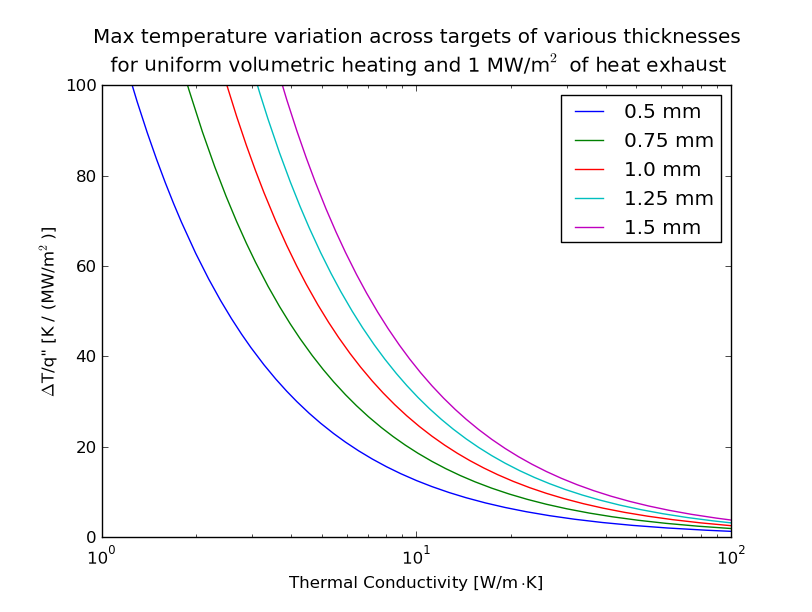
\includegraphics[width=80mm]{Figures/DeltaTvsK.png}
%\caption{ $\Delta T$(normalized to $q$) versus thermal conductivity. }
%\label{fig:DeltaT}
%\end{center}
%\end{figure}

%A plot of $\Delta$T( normalized to $q''$) versus thermal conductivity is shown in Figure \ref{fig:DeltaT}, assuming heat removal from both sides of the sample.  This plot shows that the $\Delta$T will constrain the damage rates of the samples, especially for materials with low $k$.  The heat removal limitations are better illustrated by the calculation of maximum heat flux for a given $\Delta T$, using equation \ref{eq:QMax}.

Considering thermal conductivity $k$, the limits on $\Delta$T will constrain the damage rates of the samples, especially for materials with low $k$.  These heat removal limitations are illustrated by the calculation of maximum heat flux for a given $\Delta T$, using equation \ref{eq:QMax}.

\begin{equation} 
q'' = \frac{4 \Delta T \cdot k}{t} 
\label{eq:QMax}
\end{equation} 

For this study,  $\Delta$T = 20$\;$K was used because the ASTM standards require the temperature to be reported with $\Delta $T $\pm 10\;$K for irradiation damage studies \cite{ASTME521}.  A plot of heat flux $q''$ versus $k$, with $\Delta$T = 20$\;$K is shown in Figure \ref{fig:MaxQ}.
 
\begin{figure}[htbp]
\begin{center}
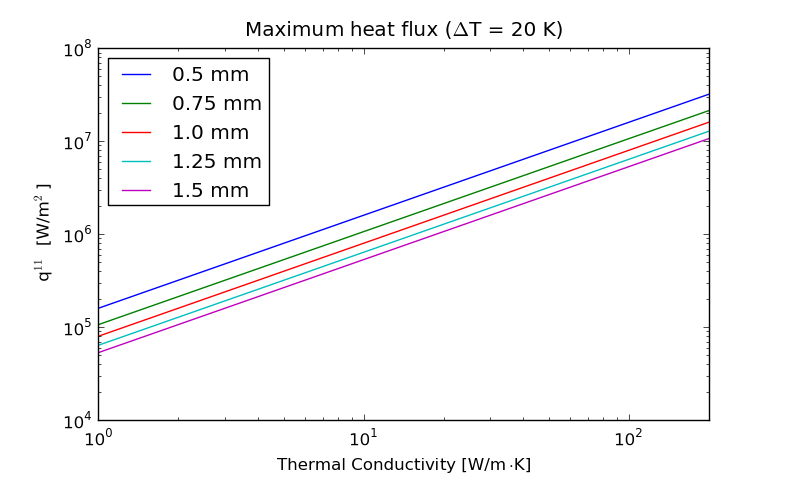
\includegraphics[width=80mm]{Figures/MaxQFluxVsK.png}
\caption{Heat flux limitations for maintaining less than $\Delta\mathrm{T} = 20\;$K across the sample.}
\label{fig:MaxQ}
\end{center}
\end{figure}

\subsection{Discussion of Operating Limits}
Combining the two constraints gives operating limits for the samples maximum damage rate.  For the heat removal constraint, a heat transfer coefficent $h$ of 25 kW/m$^2$K was assumed. This is a conservative estimate based on $h$ predicted from modeling results in Section \ref{sec:HeatRemoval} and reference \cite{Ihli}. For the $\Delta$T constraint, temperature-dependent thermal conductivity data was used from the \emph{Handbook of Heat Transfer (3rd Edition)}, Ed. Rohsenow, et al. \cite{HTHandbook}.  The resulting operating limits are summarized in Figure \ref{fig:OpLimits}.

\begin{figure}[htbp]
\begin{center}
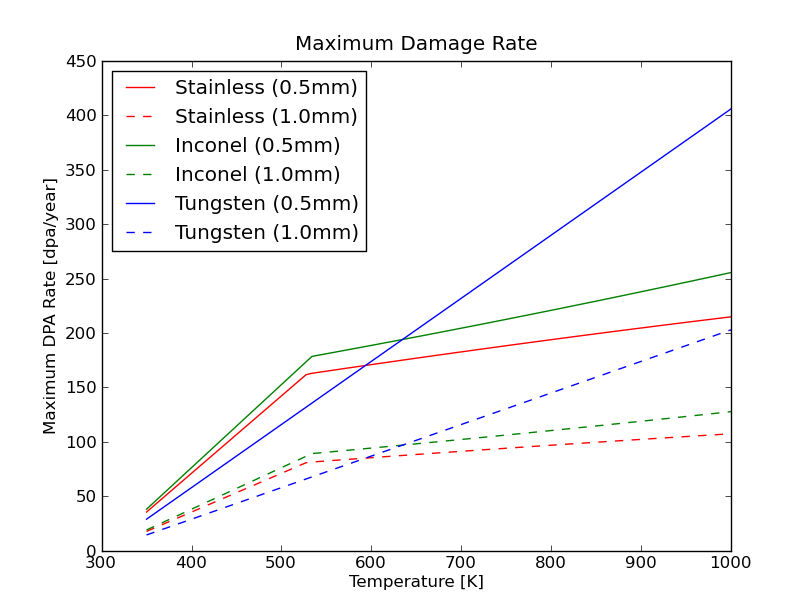
\includegraphics[width=80mm]{Figures/OpLimits.png}
\caption{Operating limits for maximizing damage rate, constrained by heat removal and $\Delta T$.}
\label{fig:OpLimits}
\end{center}
\end{figure}

Figure \ref{fig:OpLimits} demonstrates that the operating limits behave differently based on the thermal properties and the dimensions of the sample.  For refractory metals with high thermal conductivity ($>$150W/mK) such as tungsten, the heat removal is the dominant constraint on the damage rate.  However, with structural materials like Inconel and stainless steel, which have much lower thermal conductivities (10-30 W/mK), the operation is limited by heat removal at low temperature and $\Delta$T at high temperature.  Furthermore, the maximum damage rate decreases linearly with sample thickness.


%***************************************************************************
\subsection{Thermal Modeling}
\label{sec:HeatRemoval}
The primary limitation to accelerating DPA rates is heat removal from the samples.  Helium jet impingement cooling is used because of the high heat transfer coefficients $h$ that it can provide and because of experience in fusion divertor design \cite{Ihli}.  Due the large heat fluxes involved and temperature requirements of the samples, accurate modeling of heat transfer is essential for temperature control and adequate heat removal.

\begin{itemize}
\item Jet impingement cooling experience in fusion/industry.
\item Heat transfer calculation/extrapolation to show feasibility.
\item It is not unreasonable to expect adequate heat removal given the extrapolations, however further modeling is required.
\item Calculated requirements for helium flow.
\item Feasiblity of pumps / survey of required pumping technology.
\end{itemize}

\begin{figure}[htbp]
\begin{center}
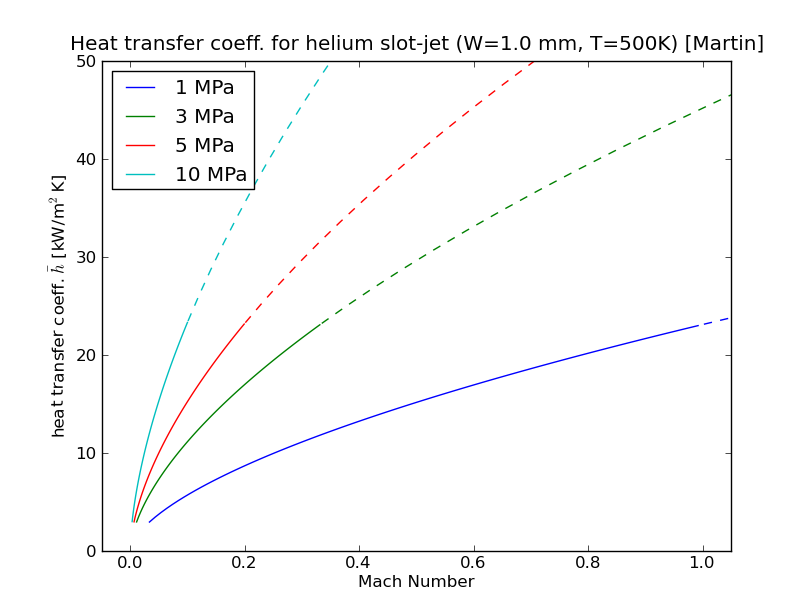
\includegraphics[width=80mm]{Figures/htc vs mach number 1mm T500K.png}
\caption{Calculated heat transfer coefficients calculated with the Martin \cite{...} correlation vs helium mach number.  The dotted region of the curves indicate extrapolations beyond the correlation's range.} 
\label{fig:SRIMDPA}
\end{center}
\end{figure}

...............................................................................\\
................................................................................\\
................................................................................\\
................................................................................\\
................................................................................\\
................................................................................\\

\subsection{Irradiated Sample Volume}
...............................................................................\\
................................................................................\\
................................................................................\\
\begin{itemize}
\item Discussion of estimated irradiated volume.
\item Possible shape and size of of samples.
\item Comparison to other techniques.
\end{itemize}
...............................................................................\\
................................................................................\\
................................................................................\\
................................................................................\\
................................................................................\\
................................................................................\\


\section{DPA Calculations} 

When simulating neutron damage, it is important to have a model for calculating the induced damage rates in materials, so that samples can be irradiated for the appropriate exposure time.  Damage rates typically decrease with energy at beam energies in the 10s of MeV, and vary significantly between materials.  Calculating these damage rates is not necessarily straightforward because of the complicated physics involved  with the production of primary knock-on  atoms (PKA), the damage cascades that follow, and the subsequent migration of vacancies and interstitials \cite{Was}. 

% A variety of methods are available to estimate DPA.  It is also frequently difficult to determine the methods used to evaluate DPA rates that are reported in various publications. This made it difficult to establish a reliable and consistent method for calculating DPA rates.  As a result, a considerable  effort was devoted to DPA calculations. 

For this study, two methods were used for calculating DPA rates. The Monte Carlo code, SRIM 2008, which includes a detailed damage calculations \cite{SRIM}, was used to calculate damage rates and an analytical model from reference \cite{Was} was used to validate the order of magnitude of the results.  

These calculations scale inversely with the displacement threshold energy $E_d$ of the material, so selection of the proper value is important.  In the literature, there is a significant variation in the values for $E_d$. Due to large uncertainties and the effects of crystal structure, it is not uncommon for quoted $E_d$ values for to vary by as much as factor of 2.   For these DPA rate calculations, $E_d$ values from the ASTM E521 \emph{Standard Practice for Neutron Radiation Damage Simulation by Charged-Particle Irradiation} \cite{ASTME521} were used. These are also given in a table in the G. Was book \cite{Was}.  

These methods give results in units of displacements per ion per unit length.  The results were converted to a more informative unit of displacement per atom (dpa) per unit time, which was then normalized to a reasonable beam current density.  This was done to provide damage rates that be easily related to the facility's performance and beam parameters 

% It was not unusual to see 25 eV listed as the $E_d$ value for a given metal in one source, and then 35 eV listed as the value in a second source. Overall, there seems to be a lot of uncertainty regarding these exact values. Obviously, it is difficult to find exact values for any specific steel or alloy, and it is assumed that $E_d$ is regarded as an estimate.% The value of $E_d$ gives an idea of how much energy incident radiation must impart in order to cause a displacement. 

\subsection{DPA Rates from SRIM 2008}

%Monte Carlo codes are typically used to make displacement calculations because of the complicated physics of damage cascades.  
Monte Carlo codes are typically used to make displacement calculations in order to capture complicated physics of damage cascades.  In this study, SRIM 2008 \cite{SRIM} was used to perform detailed damage cascade calculations using the minimum threshold energies listed in ASTM E521 \cite{ASTME521}.  The results are shown in Figure \ref{fig:SRIMDPA}. %The results of this calculation are shown in Figure \ref{fig:WasDPARate}.  
 
\begin{figure}[htbp]
\begin{center}
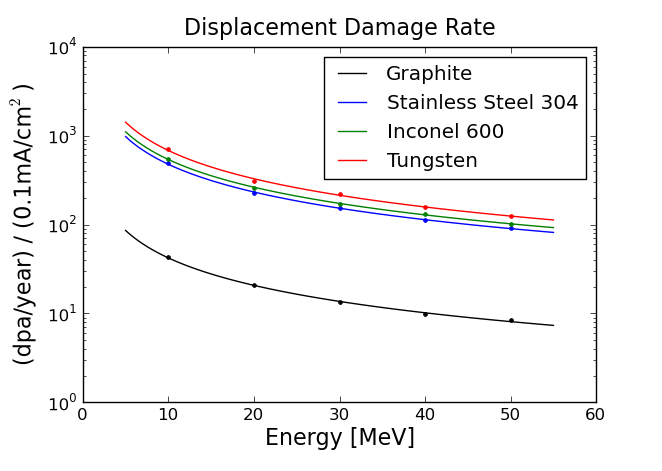
\includegraphics[width=80mm]{Figures/SRIMDPA.png}
\caption{Monte Carlo simulation results for displacement damage rates for various materials, calculated with SRIM 2008.} 
\label{fig:SRIMDPA}
\end{center}
\end{figure}
% 
%\subsection{DPA rates from analytic model}
%
%An analytical formula (equation \ref{eq:WasDPAModel}), detailed in \emph{Fundamentals of Radiation Materials Science: Metals and Alloys} was used to estimate DPA rates \cite{Was} in order to verify that the SRIM calculations yielded reasonable results.  The model gives the displacement rate $R_d$ calculated from equation \ref{eq:WasDPAModel}.
%
%\begin{equation}
%\frac{R_d}{NI} = \frac{\pi Z^2_i Z^2_2 \epsilon^4}{4 E_1 E_d} \left(\frac{M_i}{M}\right) \ln \left(\frac{\gamma E_i}{E_d}\right)  \left[\frac{\mathrm{dpa}}{\mathrm{ion/cm^2}}\right] 
%\label{eq:WasDPAModel}
%\end{equation} 
%
%(Was, 118) Here, $E_i$ is the proton energy and $E_d$ is the displacement energy. $\gamma$ = $\frac{4M_1M_2}{(M_1 + M_2)^2}$,  $\epsilon$ is the unit charge of a proton (in statCoulombs), $N$ is the number density of the sample, and $I$ is incident particle flux of the proton beam. The results of this calculation are shown in Figure \ref{fig:WasDPARate} for protons on iron.  The results of both of these calculations are within a factor of 2 for equal values of $E_d$, thus providing a check on the SRIM results.
%
%\begin{figure}[htbp]
%\begin{center}
%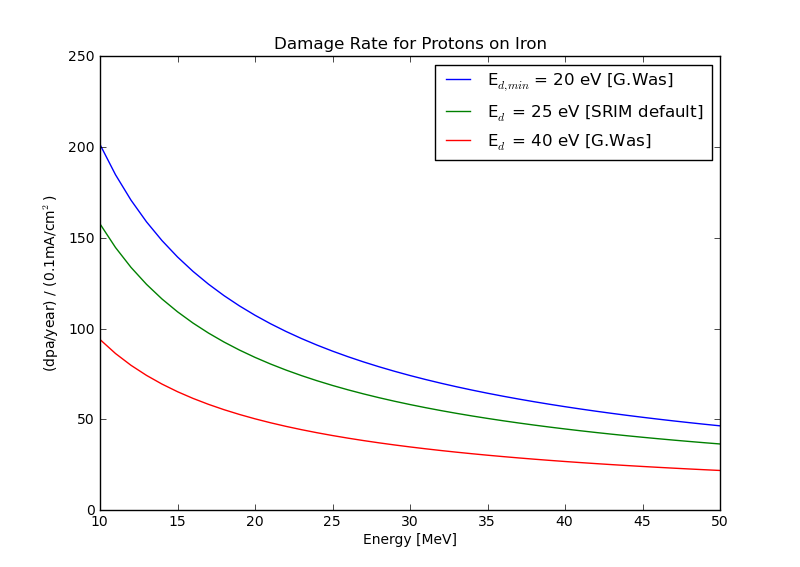
\includegraphics[width=80mm]{Figures/GWasDpaRate.png}
%\caption{DPA rates for iron calculated for various displacement threshold energies $E_d$, using the analytic model given on p.118 in Was \cite{Was}}
%\label{fig:WasDPARate}
%\end{center}
%\end{figure}

%We suspect that this formula may not be sufficient for modeling interactions between the facility proton beam and the samples, since it does not account for cascade effects. However, DPA estimations were still made for graphite, tungsten, and stainless steel (90\%Fe, 10\%Cr).  These results are shown in Figure 3; the entirety of these calculations is in the document `DPA Estimations.'

%\begin{figure}[htbp]
%\begin{center}
%\title{DPA rates versus beam energy [ergs]}
%\includegraphics[scale=0.54]{DPAgraph.jpg}
%\caption{The graph shows the DPA rates per year for (from left to right) graphite, tungsten, and stainles steel) as a function of proton beam energy in ergs. Converting the x-axis to MeV gives valus of 30.8 MeV, 61.7 MeV, and 92.5 MeV for the first three marked ticks.}
%\label{default}
%\end{center}
%\end{figure}
%For a beam energy of 35 MeV, estimated dpa/year for graphite, tungsten, and stainless steel were 17.5, 26.7, and 30.5 respectively. 

%\subsection{dpa per year, given thermal constraints} 

%We examine six materials that would be likely candidates for testing: Iron (Fe), Tungsten (W), Zirconium (Zr), Graphite (C), Silicon Carbide (SiC), and Vanadium (Va). \textbf{dpa/year} are calculated assuming (1) a maximum possible heat flux, based on heat removal capabilities within the facility and (2) the heat flux that corresponds to the maximum allowable temperature variation on the test sample.

%(1) \emph{Maximum heat flux}. We assume that the maximum volumetric heat flux we can remove with the current design of the gas-jet cooling system is 20 GW/m$^3$, or 20 MW/m$^2$.  The proton beam energy is taken at E$_i$ = 35 MeV. 

%From the equation \begin{equation} q'' / t = I\cdot S(E) \end{equation}, where q''= 20 $\cdot$ 10$^6$ W/m$^2$, t = sample thickness, I = beam density in A/m$^2$, and S(E) = the stopping power coefficient of the target sample in eV/m, we find the maximum beam current that can be incident on each sample material. From the maximum beam current, we find dpa/year according to beam energy vs. $\frac{\mathrm{dpa/s}}{\mathrm{mA/cm^2}}$ relationships determined for each material using SRIM. \cite{HaroldDPA}

%(2) \emph{Maximum temperature variation.} Based on ASTM standards, the maximum temperature variation across the sample is 20$^\circ$. \cite{ASTM} We use the following formula, 

%\begin{equation} q'' = \frac{4 \Delta T k}{t} \end{equation} 

%where $k$ is the sample's thermal conductivity and $\Delta$ T = 20. From this $q''$,  we return to equation (1) to find the new maximum beam current and the corresponding dpa/year. 

%Table 1 shows these results.\footnote{Insofar as units are concerned, note that MW/m$^3$ = Amps/m$^2$ $\cdot$ eV/m. Also note that $q''_2$ accounts for the total heat flux off both sides of the target sample. $k$ was estimated based on a temperature of about 500$^\circ$ C, since this table aims only to estimate the orders of expected dpa rates. More exact values would be needed to get a highly accurate model of a sample's thermal behavior inside the facility.}

%\begin{table}[htdp]
%\caption{DPA/year, assuming a 1 mm thick sample target}
%\begin{center}
%\begin{tabular}{c c c c c c c c c c}
%\hline
%Material & S(E)  [$\frac{\mathrm{MeV}}{\mathrm{mm}}$] & k [$\frac{\mathrm{W}}{\mathrm{mK}}$]  & $q''_1[ \frac{\mathrm{MW}}%{\mathrm{m^2}}]$ &j$_1 [\mathrm{\frac{mA}{cm^2}}]$ & dpa/y$_1$ & $q''_2 [\frac{\mathrm{MW}}{\mathrm{m^2}}]$ & j$_2 [\mathrm{\frac{mA}{cm^2}}]$ &  dpa/y$_2$\\
%\hline
%Fe & 8.741 & 80.4 & 20 & .230 & & 12.86 & .147 \\
%W & 15.07 & 173 & 20 & .1323 & 250 & 26 & .173 & 325 \\
%Zr & 6.293 & 22.6 & 20 & .318 & & 18.1 & .288\\ 
%C & 3.35 & 130 & 20 & .597 & 69 & 20.8 & .621 & 72\\
%SiC & 4.369 & 55.1& 20 & .459 & & 8.8 & .201\\ 
%Va & 6.596 & 30.7 & 20 & .353 & & 5 & .076\\
%\end{tabular}
%\end{center}
%\label{default}
%\end{table}%
%
%\begin{figure}[htbp]
%\begin{center}
%\title{Sample Thermal Conductivity versus Thickness}
%\includegraphics[scale = 0.40]{KvsT.jpg}
%\caption{Assuming the relationship $q'' = \frac{4 \Delta T k}{t}$ holds true, we take a maximum $q''$ of 20 MW/m$^2$ and a maximum $\Delta T$ of 20 $^\circ$. For these maximum possible allowances, the graph shows the relationship between \textbf{thickness $t$, in meters (y-axis)} and \textbf{thermal conductivity $k$ in W / m $\cdot$ K, on the x-axis}. At this time, 1 mm is considered to be the standard sample thickness. Most materials have a thermal conductivity below 250 W/m$\cdot$K : far more constraining will be the grain size of a material. To get the necessary 10 grains for bulk simulation, grains will need to be under 100 $\mu$m in size to remain at or below a 1 mm sample thickness. (See the materials section.) Note also that low-conductivity samples will likely need to be made thinner to ensure that the $ \Delta T$ limits are not exceeded.  }
%\label{default}
%\end{center}
%\end{figure}
%
%In discussing facility design, 1 mm is the sample thickness that is usually quoted. However, the most important thing to consider is whether the sample placed in the irradiation facility will be thick enough to simulate bulk material behavior in a reactor environment. Therefore, the thickness should be at least ten grains: for some alloys, more than 1 mm of thickness would be required; for others, a much thinner sample would suffice.
%
% For some common alloys, however, these constraints could be problematic: certain ferritic steels may have grain sizes of more than 200$\mu$m, for example, and therefore 2 mm thickness would be required to include the recommended 10 grains. Therefore, in the future, it would be helpful to (a) collect a list of common reactor steels with grain sizes $>$ 100 $\mu$m, and ensure that the current facility design would not exclude too great a number of important materials and (b) further examine the possibility of increasing the allowable thickness of samples. This could potentially be done assuming that the cooling system could handle the additional demand that would result from increasing sample thickness.
%
%Note that the thickness will affect the temperature distribution on the sample. Therefore, a sample with poor thermal conductivity but small grain size may still be testable, since the thickness will be able to be decreased from the 1 mm benchmark, and $q''$ can be increased (thus hopefully increasing the yearly dpa rate to a more acceptable number).\footnote{This implies that the target chamber design - and in particular, the sample holders - should be able to accommodate samples of varying thicknesses.}

\subsection{Discussion of Damage Simulation}

The potential differences between displacements caused by neutrons versus protons must be addressed in order to validate results from MTF.  Damage from protons is caused long range coulomb scattering in addition to large angle scattering.  Damage from neutrons however is dominated by large angle scattering causing higher average recoil energies.  These differences in recoil spectra will likely have an effect on the distribution and average length of damage cascades.  The effects on the material properties however, are unclear and require further study.

The recoil spectra for mono-energetic protons versus neutrons can have similar distributions for high energy recoils \cite{Logan}, but vary substantially for low energy recoils.  Recoils from protons typically span a broad range of energies whereas recoils from neutrons have a much narrower distribution \cite{Was}.  Despite this disparity however, since reactors typically have broad neutron spectra, their recoil spectra will also span a broad range of energies.  This means that the characteristic broad recoil spectrum from a mono-energetic proton beam could be beneficial in simulating realistic reactor conditions.  Analysis of the recoil spectra requires further study with computational codes such as MCNP and GEANT4.

\section{Beam Window}

The sample must be surrounded by high pressure helium gas to achieve sufficient helium jet impingement cooling on both sides. However, accelerators must be kept under high vacuum in order to operate.  A thin vacuum--gas boundary must therefore be designed to accommodate these requirements.  Since both the strength of the window and the beam energy loss increase with window thickness, optimization is required to minimize energy loss of the beam while maintaining its structural integrity.  The window material is also important.  It must be resilient to radiation damage, and should be made of material of low nuclear charge in order to reduce energy loss and window heating.  A schematic of the window geometry is shown in figure \ref{fig:Window}.


\begin{figure}[htbp]
\begin{center}
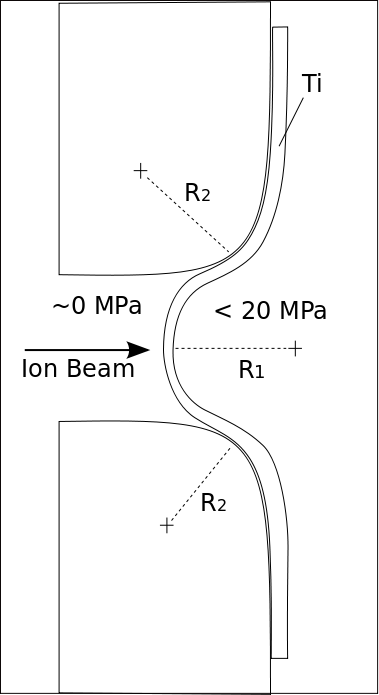
\includegraphics[width=40mm]{Figures/WindowSchematic.png}
\caption{The schematic of the beam window. The gas pressure of the window causes it to deform in the vacuum region. The edges of the supporting aperture must be smooth to minimize the shear stress at the edge of the window.}
\label{fig:Window}
\end{center}
\end{figure}

The design requires a long ($\sim$10 cm) and narrow  (1--3 mm)  window with a thickness of 10--100$\mu$m.  Since the length of the window $L$ is much longer the width $w$ of the window aperture, and the thickness $\tau$ of the window is much less than the width ($L \gg w \gg \tau$), the window can be modeled as a thin walled cylinder. The minimum thickness can thus be calculated using equation \ref{eq:ThinCylinder}, where $P_o$ is the pressure in the target chamber, $r$ is the radius of curvature of the window surface, and $\sigma$ is the stress in azimuthal direction.  

\begin{equation}
\sigma_{\theta} = \frac{P_o\cdot r}{\tau} \quad \longrightarrow \quad \tau_{min} = \frac{P_o\cdot r_{min}}{\sigma_{max}}
\label{eq:ThinCylinder}
\end{equation}

%The design requires a long ($\sim$10 cm) and narrow window (1--3 mm) with a thickness of 10--100$\mu$m.  Since the length of the window $L$ is much longer the width $w$ of the window aperture, and the thickness $\tau$ of the window is much less than the width ($L \gg w \gg \tau$) the window can be modeled as a thin walled cylinder using.  The minimum thickness can thus be calculated using equation \ref{eq:ThinCylinder} where $P_o$ is the pressure in the target chamber, $r$ is the radius of curvature of the window surface and $\sigma$ is the stress in azimuthal direction.  

\begin{table}
\begin{center}
\begin{tabular}{|c|c|c|c|c|}
  \hline
width & 5 MPa  &  10 MPa  &  15 MPa  &  20 MPa \\
$w$ [mm]  &  $\tau$ [$\mu{m}$]  &  $\tau$ [$\mu{m}$]   &  $\tau$ [$\mu{m}$]   & $ \tau$ [$\mu{m}$] \\ \hline
1 & 2.8 & 5.6 & 8.4 & 11.2 \\
2 & 5.6 & 11.2 & 16.8 & 22.3 \\
3 & 8.4 & 16.8 & 25.1 & 33.5 \\
\hline
\end{tabular}
\caption{Minimum thickness $\tau$ for a titanium beam window with $L \gg w \gg \tau $ and $\sigma_{max} = 895\;$MPa.}
\label{tab:MinThickness}
\end{center}
\end{table}

Beam windows are a well established technique for producing external (in-air) ion beams which are used extensively for ion beam analysis \cite{Doyle} and have applications in biology and medicine \cite{Maehaut}.  Since the window used for this project requires higher pressures and beam currents,  a semi-empirical design approach is preferred.  The window thickness should be chosen from the minimum calculated thicknesses from Table \ref{tab:MinThickness} and multiplied by an engineering safety factor to account for degradation due to heating and radiation damage.  Since failure of the window could have serious consequences for the vacuum system and other components, the windows dimensions should be experimentally validated.


%*******************************************************************************
\section{Time Structure of the Beam Interactions} 

Proton irradiation for simulation of damage has the benefit of very high damage rates compared to those incurred by neutrons.  Accelerated damage, however, has the potential to introduce non-linearity in the materials response due to interference between damage cascades if the damage rates are too high. 

Cyclotrons produce inherently pulsed beams, even when operating in continuous wave (CW) mode.  A 35 MeV cyclotron will typically have a frequency of $\sim$100 MHz and a duty factor of $\sim$10\%.  This makes the instantaneous damage rate higher than the time averaged damage rate by roughly a factor of 10. This could further contribute to the unrealistic damage effects.  Analysis is therefore necessary to show the constraints on  accelerating the damage rates in the samples. 

% (shown in Table \ref{tab:DamageTimes}).  

%\begin{table}[h]
%\begin{center}
%\begin{tabular}{ | c | l | }
%\hline Timescale[s] & Event \\ \hline
% & Energy transfer from incident\\ 
%$10^{-18}$ & particle: formation of primary\\
% & knock-on (PKA) atom. \\ \hline
% & Displacement of lattice atoms\\
%$10^{-13}$ & by PKA: Displacement cascade. \\ \hline
% & Energy dissipation, recombination\\
%$10^{-11}$ & and clustering: Formation  \\
% & of stable Frenkel pairs. \\ \hline
% & Thermal migration: Interstitial- \\
%$>10^{-8}$ & vacancy, recombination,clustering, \\
% &trapping, defect emission. \\ \hline
% %& Mean time between incident beam particles. \\
% %$1.6\times 10^{-16}$ & (beam current = 1mA) \\ \hline
% %& Transit time through a 1$\mu$m sample. \\
%%$10^{-14}$ & (50MeV H$^+$ ions)\\ \hline
%\end{tabular}
%%\caption{Radiation damage time scales \cite{Was}.}
%\label{tab:DamageTimes}
%\end{center}
%\end{table}

A simple but adequate approach to this issue is a comparison between the volumetric displacement rate and characteristic timescales of the cyclotron pulses and the damage cascades.  The volumetric displacement rate $R_d$ can be calculated from the DPA rate $R_{dpa}$ from equation \ref{eq:DPALimit1}.

\begin{equation}
R_{dpa}\left[\frac{\mathrm{disp}.}{\mathrm{atom}\cdot \mathrm{s}}\right] \cdot n \left[ \frac{\mathrm{atom}}{\mathrm{m}^3} \right] = R_d \left[ \frac{\mathrm{disp}}{\mathrm{m}^3\cdot \mathrm{s}} \right ] 
\label{eq:DPALimit1}
\end{equation}

The mean time $\tau$ between the displacements can then be calculated using the volume of a displacement cascade, which can be approximated from the range and lateral straggling of the PKAs.  The range of the PKA, $R_{pka}$, can be determined from the from elastic scattering kinematics. Range data and the lateral straggling $L_{pka}$ can be calculated with SRIM 2008 \cite{SRIM}.  For a conservative estimate, a sphere can be used for the damage volume  $V_{sphere} = 4/3 \pi R_{pka}^3$.  For a more realistic estimate, the damage cascade can be modeled as a cone with volume $V_{cone} =\frac{1}{3} \pi R_{pka}^2 L_{pka}$.  The mean time between displacements in the maximum energetically allowed cascade volume is shown as a function of beam energy in figure \ref{fig:DisplacementTime}.  The relevant damage timescales are also superimposed.

\begin{figure}[htbp]
\begin{center}
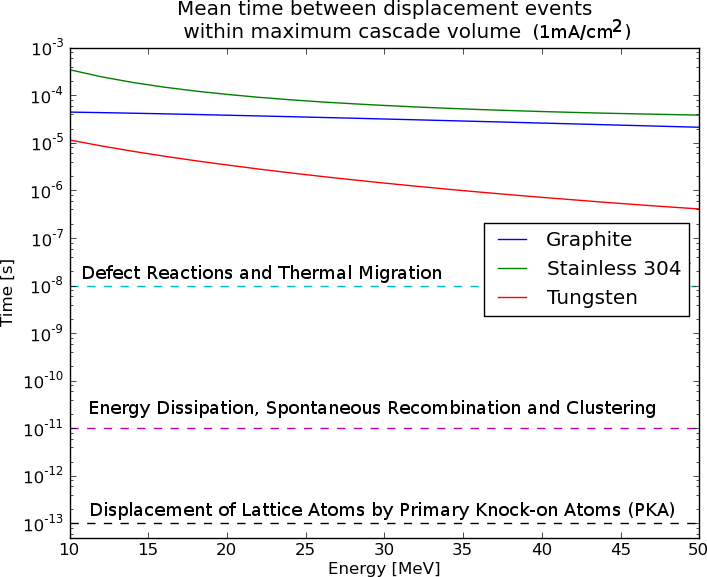
\includegraphics[width=80mm]{Figures/MeanDamageTime.png}
\caption{Mean time between displacements events per cascade volume is shown assuming a conical volume and an instantaneous beam current density of 1mA/cm$^2$. This demonstrates that }
\label{fig:DisplacementTime}
\end{center}
\end{figure}

For a modest time averaged beam current density of 0.1 mA/cm$^2$ corresponding to 1 mA/cm$^2$ of instantaneous current density, the time between displacements in a given cascade volume $\tau_d$ is on the order of micro-seconds or longer.  This means that after the initiation of a damage cascade, all of the damage processes, including the formation of a PKA, its energy dissipation, and finally recombination and thermal migration of defects, have time to reach equilibrium before the next cascade is initiated within that volume.  Similarly, the beam cyclotron period is roughly 10$^{-8}$ seconds, which is also much shorter than $\tau_d$.  

Since the displacement timescale within a cascade volume $\tau_d$ is at least two orders of magnitude longer than the damage processes involved, it is unlikely that overlapping damage cascades from the accelerated damage rate or the beam's time structure will have any affect on the damage physics.

%Shown here are two plots of the average time between displacements within a damage cascade volume.  This volume can be calculated simply as a sphere with the radius = maximum PKA range (conservative estimate).  Alternatively, the cascade volume can be estimated, perhaps more accurately, as a come with height = maximum PKA range with the radius being equivalent to the lateral straggling.  As for the diffusion length/time scales for the vacancies and interstitials, they are probably highly temperature dependent and difficult to quantify at this time.
%
%\begin{figure}[htbp]
%\includegraphics[scale=.70]{MeanTimeConVol.jpg}
%\caption{MEAN TIME CONICAL VOLUME}
%\label{default}
%\end{figure}
%
%\begin{figure}[htbp]
%\includegraphics[scale=.70]{MeanTimeSphVol.jpg}
%\caption{MEAN TIME SPHERICAL VOLUME}
%\label{default}
%\end{figure}


%*******************************************************************************

\section{Future work}

\begin{itemize}
\item Detailed engineering design
\item Further simulation of damage physics in the 35MeV energy range
\item Activation and shielding analysis of the facility
\item Experimental and CFD modeling of heat removal 
\end{itemize}

................................................................................\\
................................................................................\\
................................................................................\\

\section{Conclusions}

................................................................................\\
................................................................................\\
................................................................................\\


\begin{itemize}
\item Summary
\item Discussion of advantages
\item Discussion of technical risk
\end{itemize}

................................................................................\\
................................................................................\\
................................................................................\\


%% References using BibTeX database:

\onehalfspacing

\bibliographystyle{model1-num-names}
\bibliography{MTFpaper}

\end{document}

